\documentclass{article}
\usepackage[utf8x]{inputenc}
\usepackage{ucs}
\usepackage{amsmath} 
\usepackage{amsfonts}
\usepackage{marvosym}
\usepackage{wasysym}
\usepackage{upgreek}
\usepackage[english,russian]{babel}
\usepackage{graphicx}
\usepackage{float}
\usepackage{textcomp}
\usepackage{hyperref}
\usepackage{geometry}
  \geometry{left=2cm}
  \geometry{right=1.5cm}
  \geometry{top=1cm}
  \geometry{bottom=2cm}
\usepackage{tikz}
\usepackage{ccaption}
\usepackage{multicol}

\hypersetup{
   colorlinks=true,
   citecolor=blue,
   linkcolor=black,
   urlcolor=blue
}

\usepackage{listings}
%\setlength{\columnsep}{1.5cm}
%\setlength{\columnseprule}{0.2pt}

\usepackage[absolute]{textpos}

\usepackage{colortbl,graphicx,tikz}
\definecolor{X}{rgb}{.5,.5,.5}


\begin{document}
\pagenumbering{gobble}
\lstset{
  language=C,                % choose the language of the code
  basicstyle=\linespread{1.1}\ttfamily,
  columns=fixed,
  fontadjust=true,
  basewidth=0.5em,
  keywordstyle=\color{blue}\bfseries,
  commentstyle=\color{gray},
  stringstyle=\ttfamily\color{orange!50!black},
  showstringspaces=false,
  numbersep=5pt,
  numberstyle=\tiny\color{black},
  numberfirstline=true,
  stepnumber=1,                   % the step between two line-numbers.        
  numbersep=10pt,                  % how far the line-numbers are from the code
  backgroundcolor=\color{white},  % choose the background color. You must add \usepackage{color}
  showstringspaces=false,         % underline spaces within strings
  captionpos=b,                   % sets the caption-position to bottom
  breaklines=true,                % sets automatic line breaking
  breakatwhitespace=true,         % sets if automatic breaks should only happen at whitespace
  xleftmargin=.2in,
  extendedchars=\true,
  keepspaces = true,
}
\lstset{literate=%
   *{0}{{{\color{red!20!violet}0}}}1
    {1}{{{\color{red!20!violet}1}}}1
    {2}{{{\color{red!20!violet}2}}}1
    {3}{{{\color{red!20!violet}3}}}1
    {4}{{{\color{red!20!violet}4}}}1
    {5}{{{\color{red!20!violet}5}}}1
    {6}{{{\color{red!20!violet}6}}}1
    {7}{{{\color{red!20!violet}7}}}1
    {8}{{{\color{red!20!violet}8}}}1
    {9}{{{\color{red!20!violet}9}}}1
}

\section*{Домашнее задание: Сортировки}
\subsection*{Сложность алгоритмов}
\subsubsection*{Чему равна средняя вычислительная сложность следующих операций?}
\begin{enumerate}
\item Поиск элемента в массиве размера $N$
\item Поиск элемента в отсортированном массиве размера $N$ (бинарный поиск)
\item Добавление элемента в начало массива размера $N$
\item Добавление элемента в конец массива размера $N$ (в предположении, что \texttt{capacity} > \texttt{size})
\item Добавление элемента в динамический(саморасширяющийся) стек размера $N$
\item Сортировка выбором массива размера $N$
\item Сортировка пузырьком массива размера $N$
\item Быстрая сортировка массива размера $N$
\item Сортировка подсчётом массива размера $N$, если максимальный элемент массива равен $K$
\item Цифровая сортировка массива размера $N$, если максимальный элемент массива равен $K$
\item Сортировка Bogosort массива размера $N$
\item Сортировка слиянием массива размера $N$
\item Сложение матриц размера  $N \times N$
\item Простой алгоритм умножения матриц размера  $N \times N$ (строка на столбец)
\item Сложение двух чисел длиной в $N$ цифр ($N$ может быть большим)
\item Простой алгоритм умножения(столбиком) двух чисел длиной в $N$ цифр ($N$ может быть большим)
\item Простой алгоритм проверки числа на простоту перебором от двух до корня этого числа. Число состоит из $N$ цифр в десятичной записи ($N$ может быть большим)
\item $\!\!\!\!{^*}$ Добавление элемента в двоичную кучу размера $N$
\item $\!\!\!\!{^*}$ Удаление элемента из двоичной кучи размера $N$
\end{enumerate}

\newpage
\section*{Быстрая сортировка - Quicksort}
\begin{multicols}{2}
\begin{lstlisting}
#include <stdio.h>
#include <stdlib.h>
#define N 30

void quicksort(int array[], int lo, int hi)
{
    if (hi - lo > 1)
    {
        int j = lo;
        int pivot = array[hi - 1];
        for (int i = lo; i < hi; i++)
            if (array[i] <= pivot)
            {
                int temp = array[i];
                array[i] = array[j];
                array[j] = temp;
                j++;
            }

        quicksort(array, lo, j - 1);
        quicksort(array, j, hi);
    }
}

void print(int array[], int n)
{
    for (int i = 0; i < n; i++)
        printf("%d ", array[i]);
    printf("\n");
}

int main()
{
    int numbers[N];
    for(int i = 0; i < N; i++)
        numbers[i] = rand() % 100;
    
    print(numbers, N);
    quicksort(numbers, 0, N);
    print(numbers, N);
}
\end{lstlisting}
\vfill\null
\columnbreak
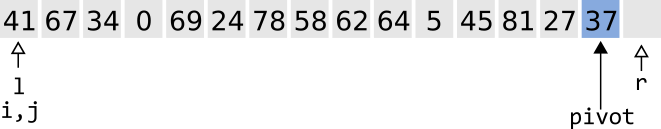
\includegraphics[scale=0.53]{../images/qs2.png}
\\
\\
\\
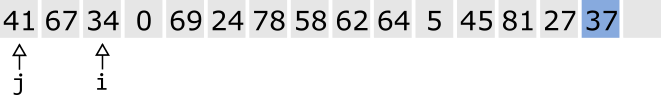
\includegraphics[scale=0.53]{../images/qs4.png}
\\
\\
\\
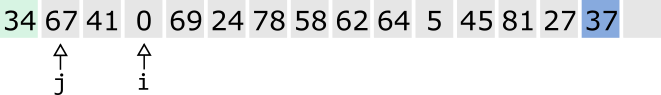
\includegraphics[scale=0.53]{../images/qs5.png}
\\
\\
\\
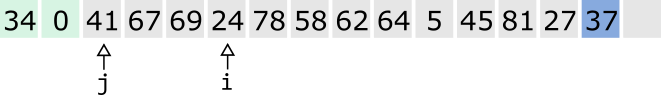
\includegraphics[scale=0.53]{../images/qs6.png}
\\
\\
\\
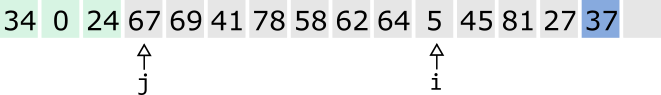
\includegraphics[scale=0.53]{../images/qs7.png}
\\
\\
\\
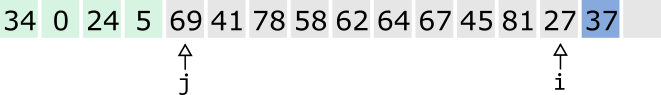
\includegraphics[scale=0.53]{../images/qs8.png}
\\
\\
\\
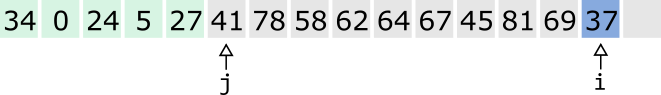
\includegraphics[scale=0.53]{../images/qs9.png}
\\
\\
\\
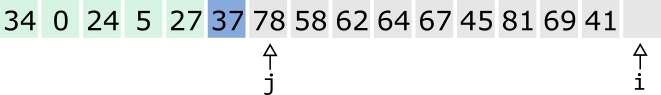
\includegraphics[scale=0.53]{../images/qs10.png}
\\
\\
\\
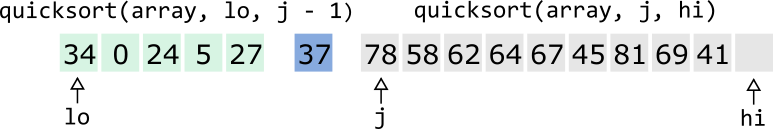
\includegraphics[scale=0.47]{../images/qs11.png}
\end{multicols}
\newpage
\textbf{Звёзды:} В файле \texttt{hipstars.csv} содержится информация о ближайших звёздах. Данные взяты из каталога Hipparcos. В каждой строке - информация об одной звезде:
\begin{enumerate}
\item \texttt{hip} - номер звезды в каталоге Hipparcos. Обратите внимание, что не все звёзды из каталога присутствуют в файле.
\item \texttt{proper\_name} - традиционное имя звезды(строка не более чем 20 символов). Большинство звёзд имён не имеют и называются просто по номеру, например HIP 3345. Если у звезды имени нет, то в этом поле стоит прочерк \texttt{-\,-}.
\item \texttt{right\_ascension} и \texttt{declination} - прямое восхождение и склонение определяют положение звезды на небе. Аналог широты и долготы.
\item \texttt{magnitude} - Звёздная величина - яркость звезды с точки зрения земного наблюдателя. Чем меньше, тем звезда ярче, шкала логарифмическая. Видимые глазом звёзды имеют звёздную величину 6 и ниже. Бетельгейзе $= 0.45$ Сириус $= -1.44$. Луна $= -12.7$. Солнце $= -26.7$. 
\item \texttt{absolute\_magnitude} Абсолютная звёздная величина - яркость звезды с точки зрения наблюдателя, находящегося на растоянии в 10 парсек от этой звезды. Бетельгейзе $= -5.47$. Сириус $= 1.45$. Солнце $= 4.85$. 
\item \texttt{spectral\_type} - спектральный класс звезды(строка не более чем 15 символов). 
\item \texttt{x}, \texttt{y} и \texttt{z} - Координаты звёзды в системе отсчёта, связанной с Землёй. Единица измерения - парсеки. \\
$1$ парсек = $3.26$ световых года = $206265$ расстояний от Земли до Солнца = $3 \cdot 10^{16}$ метров.
\item \texttt{constellation} - Созвездие (первые три буквы) или \texttt{NO}, если звезда не входит ни в какое созвездие.
\end{enumerate}
\begin{itemize}
\item Опишите структуру \texttt{Star}, которая будет предназначена для хранения информации об одной звезде.
\item \textbf{Считываем звёзды:}\\ Создайте массив из структур \texttt{Star} подходящего размера и считайте все данные из файла в массив. Файл содержит информацию о $117955$ звезде, так что массив нужно создавать в куче (с помощью \texttt{malloc}). Для считывания используйте функцию \texttt{fscanf} из библиотеки \texttt{stdio.h}. Пример считывания:
\begin{lstlisting}
#include <stdio.h>

int main()
{
    // Открываем файл input.txt на чтение("r"). Для открытия на запись - "w"
    FILE* f = fopen("input.txt", "r");
    fscanf(f, < тут всё то же самое, что и у обычного scanf >)
    // ...
    fclose(f);
}
\end{lstlisting}
Учтите, что спецификатор \texttt{\%s} считывает строку до пробела. Чтобы считать строку до запятой используйте спецификатор \texttt{\%[\textasciicircum,]} - при этом \texttt{s} на конец спецификатора ставить не надо.\\
Можно посмотреть на пример в файле \texttt{sort\_cities.c}.

\item \textbf{Сохраняем звёзды:}\\ Написать функцию \texttt{void save\_stars(char filename[], Star array[], int n)}, которая будет сохранять города из массива \texttt{array} в файл, чьё название хранится в переменной \texttt{filename}. Например, при вызове \texttt{save\_stars(``output.txt'', stars, n);} массив \texttt{stars} должен сохраниться в файл \texttt{output.txt}.

\item \textbf{Сортировка по видимой с Земли яркости:}\\ Создайте функцию \texttt{quicksort\_magnitude}, чтобы она принимала на вход массив из структур \texttt{Star} и сортировала их по возрастанию звёздной величины. Проверьте функцию в \texttt{main}, отсортировав структуру и сохранив её в файл \texttt{sorted\_by\_magnitude.txt} с помощью функции \texttt{save\_stars}.

\if false
\item \textbf{Сортировка по яркости:}\\ Создайте функцию \texttt{quicksort\_absmagnitude}, чтобы она сортировала массив звёзд по их светимости - от самой яркой к самой тусклой. Проверьте функцию в \texttt{main}, отсортировав массив и сохранив его в файл \texttt{sorted\_by\_absmagnitude.txt}.
\fi

\item \textbf{Сортировка по расстоянию:}\\ Создайте функцию \texttt{quicksort\_distance}, чтобы она сортировала массив звёзд по расстоянию от Земли. Проверьте функцию в \texttt{main}, отсортировав структуру и сохранив её в файл \texttt{sorted\_by\_distance.txt}.

\item \textbf{Сортировка по температуре:}\\ Создайте функцию \texttt{quicksort\_temperature}, чтобы она сортировала массив звёзд по температуре поверхности. Темературу можно сравнить по первым двум символам спектра. Первый символ - спектральный класс звезды - от горячих к холодным: \texttt{O->B->A->F->G->K->M}. Второй символ - подкласс - число от 0 до 9, чем меньше, тем горячее. Проверьте функцию в \texttt{main}, отсортировав структуру и сохранив её в файл \texttt{sorted\_by\_temperature.txt}.

\item \textbf{Функция-компаратор:}\\ Объедините три предыдущие функции в одну с использованием функции-компаратора. Нужно написать функцию \texttt{void quicksort(Star array[], int lo, int hi, int (*cmp)(Star* a, Star* b))}, которая будет сортировать звёзды, основываясь на функции-компараторе \texttt{cmp}. Можно посмотреть на пример в файле \texttt{sort\_cities\_funcpointer.c}.
\end{itemize}


\subsection*{Сегменты памяти. Указатели на функцию.}
\begin{center}
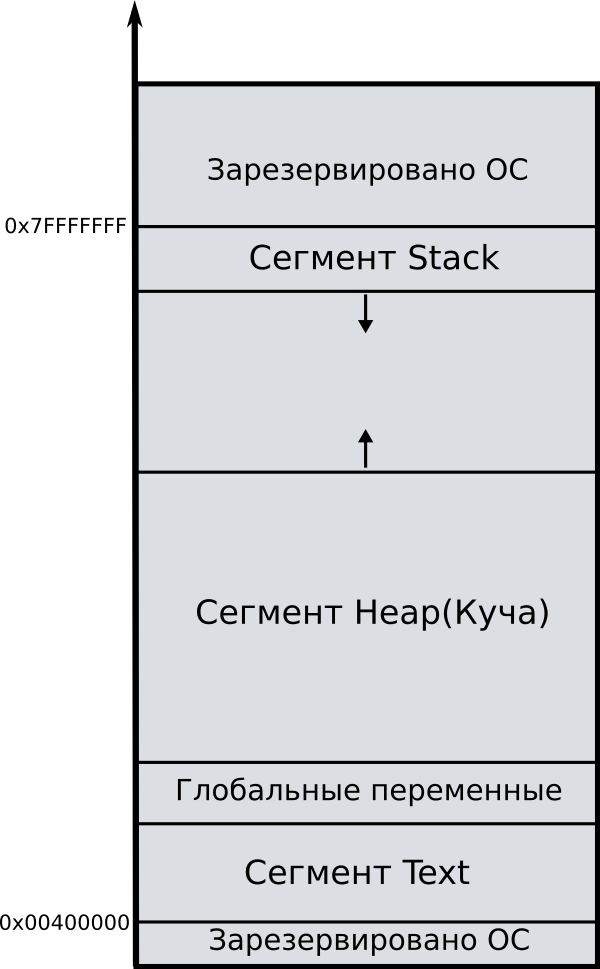
\includegraphics[scale=1.35]{../images/memory_layout.png}
\end{center}
\begin{enumerate}
\item \textbf{Сегмент памяти Стек (Stack)} \\
\begin{itemize}
\item При обычном объявлении переменных и массивов все они создаются в стеке: \texttt{int a;} или \texttt{int array[10];}
\item Память на эти переменные выделяется в начале функции и освобождается в конце функции.
\item Маленький размер (несколько мегабайт)
\item Быстрее чем куча
\end{itemize}
\item \textbf{Сегмент памяти Куча (Heap)} \\
\begin{itemize}
\item \texttt{malloc} выделяет память в Куче. \texttt{int* p = (int*)malloc(10 * sizeof(int));}
\item Память выделяется при вызове \texttt{malloc} и освобождается при вызове \texttt{free}.
\item Размер ограничен свободной памятью - гигабайты.
\item Медленней чем стек
\end{itemize}
\item \textbf{Сегмент памяти Text} \\
\begin{itemize}
\item В этом сегменте хранится машинный код программы (код на языке C, сначала, переводится в код на языке Ассемблера, а потом в машинный код).
\item Адрес функции - адрес первого байта инструкций в этом сегменте.
\end{itemize}
\end{enumerate}

Пример работы с указателем на функцию:
\begin{lstlisting}
#include <stdio.h>

void print(int a)
{
    printf("%d\n", a);
}
int main ()
{
    // Создадим указатель на функцию
    void (*p)(int a) = print;
    
    // Теперь с p можно работать также как и с print
    p(123);
}
\end{lstlisting}
Подробней в файле \texttt{funcpointer.c}.

\subsection*{Стандартная функция qsort()}

В библиотеке \texttt{stdlib.h} уже реализована функция \texttt{qsort}, которая сортирует произвольные элементы, используя быструю сортировку. Пример использования этой функции:
\begin{lstlisting}
#include <stdio.h>
#include <stdlib.h>

int cmp(const void* a, const void* b)
{
    // В этот компаратор передаются указатели на void,
    // Поэтому их нужно привести в нужный нам тип:
    int* pa = (int*)a;
    int* pb = (int*)b;
    return (*pa - *pb);
}

int main ()
{
    int arr[] = {163, 624, 7345, 545, 41, 78, 5, 536, 962, 1579};
    qsort(arr, 10, sizeof(int), cmp);
    // qsort( массив, количество элементов, размер каждого элемента, компаратор )
   
    print_array(10, arr);
}
\end{lstlisting}
\subsubsection*{Задачи:}
\begin{itemize}
\item Задачи от qsort1 до qsort9, кроме qsort6 и qsort7 на judge.mipt.ru, контест ``Задание 1.3 (структуры и указатели)''
\end{itemize}




\end{document}